\documentclass[a4paper,11pt]{article}

\usepackage[paper=a4paper,left=30mm,width=150mm,top=25mm,bottom=25mm]{geometry} 
\usepackage{fullpage}

\usepackage{amsmath}
\usepackage{amssymb}
\usepackage{graphicx}
\usepackage{gensymb}
\usepackage{enumitem}
\usepackage{setspace} % This is used in the title page
\usepackage{graphicx} % This is used to load the crest in the title page
\usepackage{subcaption}


\usepackage{afterpage}
\usepackage[hidelinks]{hyperref}


\usepackage{subfig}



\usepackage[hidelinks]{hyperref}

\usepackage{booktabs}

\usepackage[parfill]{parskip}

\graphicspath{{./Figures/}}

\usepackage{titlesec}

\begin{document}

% Set up a title page
\thispagestyle{empty} % no page number on very first page
% Use roman numerals for page numbers initially
\renewcommand{\thepage}{\roman{page}}

\begin{spacing}{1.5}
\begin{center}
{\Large \bfseries
Faculty of Information Technology\\
Monash University}

\vspace*{30mm}


\includegraphics[width=5cm]{MonashCrest}

\vspace*{15mm}

{\large \bfseries
Literature Review --- Semester 2, 2014
}

\vspace*{10mm}

{\LARGE \bfseries
Isolated Region Spatial Query
}

\vspace*{20mm}

{\large \bfseries
Jian Loong Liew 22545727

\vspace*{20mm}

Supervisor: Associate Professor David Taniar
}

\end{center}
\end{spacing}

\newpage

\tableofcontents

\newpage
\setcounter{page}{1}
\renewcommand{\thepage}{\arabic{page}}

\section{Introduction} 

A spatial query is a query that returns features based on their spatial relationship with a query geometry. The query of interest here is the \textit{Isolated Region} query. This is a distinctive spatial query in terms of its requirements and the name of it is coined from its requirements. The objective of this query is to find a region where an object can be placed so that it is not in the state of \textit{isolation} and yet still be in the state where it is in a \textit{crowd}. The input of this query will be a set of points, $S = \{p_1,....,p_n\}$ where each point represents an object of interest (OOI). The output of this query will be a region where any object placed within it satifies the criteria. 

This query should always pick the best region where the object can be placed in.

This query consist of the combination of two requirements which are:
\begin{itemize}
	\item The object must not be in the state of isolation.
	\item The object must be in the state where it is in a crowd.
\end{itemize}

Before attempting to go further the conditions of each scenario will be further defined. 

Based on Figure \ref{fig:1OOI}, it can be can seen that when only 1 object is used as the input, the conditions are quite clear. Assuming this object A, has a region of influence denoted by a circle around it, so any object placed inside the circle will be under its zone of influence. IT is quite clear that we can place any object that satisfies the condition in this scenario quite easily, because any object placed just outside the circle would be considered to be in the crowd and not isolated. 

\begin{figure}[h]
\centering
\begin{subfigure}{.4\textwidth}
  \centering
  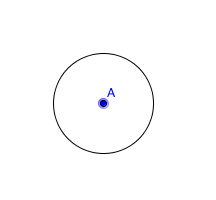
\includegraphics[width=.4\linewidth]{1OOI}
  \caption{A subfigure}
  \label{fig:1OOI}
\end{subfigure}%
\begin{subfigure}{.4\textwidth}
  \centering
  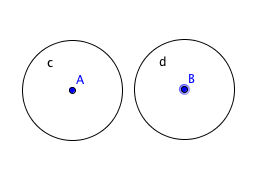
\includegraphics[width=.4\linewidth]{2OOI}
  \caption{A subfigure}
  \label{fig:2OOI}
\end{subfigure}
\caption{}
\label{fig:Condition}
\end{figure}

Based on Figure \ref{fig:1OOI}, it can be can seen that when only 1 object is used as the input, the conditions are quite clear. Assuming this object A, has a region of influence denoted by a circle around it, so any object placed inside the circle will be under its zone of influence. IT is quite clear that we can place any object that satisfies the condition in this scenario quite easily, because any object placed just outside the circle would be considered to be in the crowd and not isolated. 

\begin{figure}[h]
\centering
\begin{subfigure}{.4\textwidth}
  \centering
  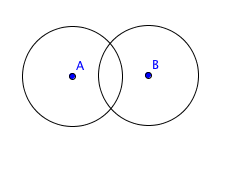
\includegraphics[width=.4\linewidth]{2OOIClose}
  \caption{A subfigure}
  \label{fig:1OOI}
\end{subfigure}%
\begin{subfigure}{.4\textwidth}
  \centering
  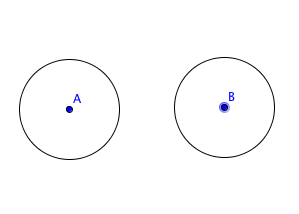
\includegraphics[width=.4\linewidth]{2OOIFar}
  \caption{A subfigure}
  \label{fig:2OOIFar}
\end{subfigure}
\caption{}
\label{fig:Condition}
\end{figure}


However this situation becomes more complex when the number of object that are the input are increased. Based on Figure \ref{fig:2OOI}, it can be seen that with 2 objects as the input, the situation of being crowded will be changed. There are also many variations of how these 2 inputs can be. For example, if the distance between these two objects are changed, the state of being in the \textit{crowd} will be different. This is because as it moves further it will be in a state of isolation. The main question here, would be how far out before it considered to be in the isolated state.

\begin{figure}[h]
\centering
\begin{subfigure}{.4\textwidth}
  \centering
  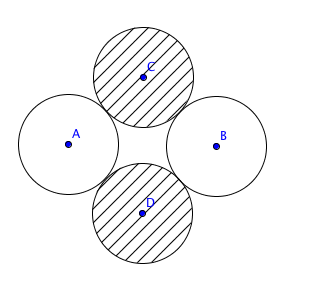
\includegraphics[width=.4\linewidth]{2OOICloseSolution}
  \caption{A subfigure}
  \label{fig:2OOICloseSolution}
\end{subfigure}%
\begin{subfigure}{.4\textwidth}
  \centering
  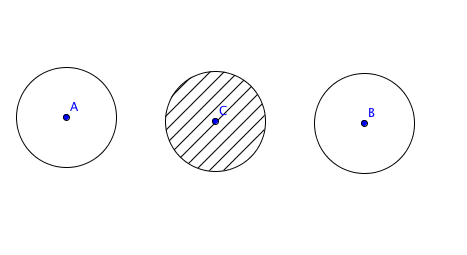
\includegraphics[width=.4\linewidth]{2OOIFarSolution}
  \caption{A subfigure}
  \label{fig:2OOIFarSolution}
\end{subfigure}
\caption{}
\label{fig:Condition}
\end{figure}

In Figure \ref{fig:2OOICloseSolution}, it can be seen that the state of being crowded will be in 2 possible place represented by C and D. This is because both of these states are similar in nature. This however is not true when the two objects are far apart. In Figure \ref{fig:2OOIFarSolution}, it is the clear that the crowded state can be satisfied by placing the object in the middle between these two objects. However this situation is not as simple as it seems, because the as two objects move futher away, it is the clear placing the object in between these two will not satisfy the condition of being the crowd. 

This situation further increases in complexity as the number of objects are increased. For example, when the number of input objects are 3, there are more possible variations to this scenario. 


Previous works has been done in order to satisfy the requirements invidually,  however no work has been done where the two constraints are placed together. Placing the two requirements together changes the way the query needs to be processed and thus this literature review aims to explore the various algorithms and approaches that can be used to solve the query. 

The definitions of the terms used are as follow.

\textbf{Definition 1} \textit{The state of being a crowd is where the query point is the zone of influence of the maximum number of objects of interest. However, in this query the condition of being in the crowd must be relaxed in order to provide a beneficial solution. Thus, being in a crowd means that the query point must be near the zone of influence of the maximum number of objects.
}

\textbf{Definition 2} \textit{The state of isolated or isolation means that the object is not under the influence of any objects of interest. This means that it has the least numbers nearest neighbours. }

\textbf{Definition 3} \textit{An Isolated Region is where the object is far away from any related object.}

\textbf{Definition 4} \textit{A safe region is an area where the query point can move freely without effecting the query result. For this query, the safe region is where an object can be placed so that it does not violate the conditions.}

\textbf{Definition 5} \textit{A zone of influence is a region where by any points or locations or coordinates or pixels in this region will consider this object as its closest object, compared to any other object.}

\subsection{Formulating of Definitions}

Here the state of being in the \texitit{``crowrd''} will be detailed. For example, if only one query point is given as the input where $S= \{ p_1\}$, the condition of the crowd needs to be defined. 



With that, the formalisation of the \textit{Isolated Region} query is as follows. Given a set of points, $p_1,....,p_n$, which are the input. The output of this will be a region in which, it is a safe zone which obeys the two requirements in which the state of any object placed within this safe zone will be in the state of being in a crowd and isolated. This output region maybe of of any shape.

Xuan in ~\cite{Xuan2012} formalised the definition of an \textit{Optimum Region} in which, ``Given a finite set of point objects and a positive value \textit{r}, the optimum region includes all points which can cover the maximum number of objects in the finite set as the center of a circle with radius r.''. This query will satisfy the requirement where the region will has the maximum number of nearest neighbours, however the input of this query will require the value \textit{r}.

Korn and Muthukrishan in~\cite{korn2000influence} formalised the notion of influence based on reverse nearest neighbour queries and its variants. This was called \textit{Influence Set}. This is because the reverse nearest neighbour is not symmetric. However. this concept of influence is often changed depending the application at hand and difficult to formalise. 

Cheema et al (2011), suggested a more generic concept called \textit{influence zone} and showed that the influence zone can be used to efficiently compute the influence sets. This influence zone has various applications in location based services and decision support systems. This is because the influence zone may be used for market analysis as well as targeted marketing~\cite{cheema2011influence}. This concept is more generic compared to the notation of influence set proposed by Korn et al (2000). 


\section{Related Works}

~\cite{guting1994introduction}

~\cite{berchtold1998fast}.

\begin{itemize}
	\item Reverse Nearest Neighbour by Korn et al. (2000)~\cite{korn2000influence}
	\item Group Nearnest Neighbour by Papadias et al. (2004)~\cite{papadias2004group}.
	\item Group Nearest Group by Deng et al. (2012)~\cite{deng2012group}
	\item Optimum Region by Xuan (2012)~\cite{Xuan2012}
\end{itemize}

In order to process the various queries in the spatial road network are as follows

\begin{itemize}
	\item Voronoi Diagrams 
	\item VN$^3$ ~\cite{kolahdouzan2004voronoi}
	\item Network Voronoi Diagram~\cite{xuan2009network}
\end{itemize}


\subsection{Overview of Spatial Queries}

This diagram is based on deriving information from ~\cite{taniar2013taxonomy}.

\section{Nearest Neighbour}

~\cite{jensen2003nearest}

~\cite{preparatat1985computational}

The nearest neighbour problem is considered to be one of the best known problems in computer science. 

~\cite{roussopoulos1995nearest}

\subsection{Range Euclidean Restriction}

~\cite{papadias2003query}. 

\subsection{Aggregate Nearest Neighbour Query}

Aggregate nearest neighbour queries returns the object that minimizes an aggregate distance function with respect to a set of query points~\cite{yiu2005aggregate}. A scenario for ANN is as follows: Assumming for example, $n$ users at location $(q_1,....,q_2)$. An ANN query outputs the facility that minimises the sum of distances that the users have to travel in order to meet there~\cite{papadias2005aggregate}. Thus, the input for an ANN query will be the set of static data points given to it.

\subsection{Constrained Nearest Neighbour}

~\cite{ferhatosmanoglu2001constrained}.

\subsection{Reverse \textit{k}-Nearest Neighbour (R\textit{k}NN)}

The goal of a reverse \textit{k}-nearest neighbour query is to identify the ``influence'' of query object on the whole data set~\cite{achtert2006efficient}. 

A Reverse Nearest Neighbour (RNN) search is a method to retrieve all objects that consider the query point as the nearest neighbour. An example would be like when a marketing application in which the issue is to determine the business impact of opening an outlet of Company \textit{A} at a given location. A simple task is to determine the segment of \textit{A}'s customer who would be likely to use this new facility~\cite{korn2000influence}. Korn et al (2000) broken this down into two cases which are static and dynamic cases and also formalised a novel notion of influence based on reverse nearest neighbour queries and its variants. Influence sets based on reverse nearest neighbour (RNN) queries seem to caputre the notion of influence based on the example stated by them.



This methodology to generate the influence zone of each location will be used in order to generate the influnce zone of each object of interest. 


\section{Constrained Range Search}

~\cite{xuan2011constrained}.

~\cite{kolahdouzan2004voronoi}

~\cite{zhao2008incremental}

~\cite{hu2006fast}

\section{Reverse Region Query}

The input of this are objects and the output of this query is a region. 

\section{Group Nearest Neighbour} 

This was proposed by Papadias et al~\cite{papadias2004group}. It is considered to be a novel form of Nearest Neighbour search. The GNN query is different from the traditional \textit{k}nn query which only specifies a single query point, the GNN query has multiple query points. The input of this problem consist of  a set of $P=\{p_1,...,p_n\}$ of static data points in multi dimensional space and a group of query points. $Q=\{q_1,...,q_n\}$. The ouput of this contains the $k>1$ data points~\cite{papadias2004group}. 

An example scenario for the GNN would would be to select a meeting place from all available meeting places. For example, for three executive directors who are located in three different places, to meet at the closest meeting place~\cite{taniar2013taxonomy}.

This is considered to be an expensive problem by definition because of the number of data points as well as query points it needs to process as it is considerably more complex than the traditional \textit{k}nn queries. The reason for this complexity is mainly due to two reasons~\cite{li2005two}. The first is because there are multiple query points being specified which requires more distance computation and the other is because the fact that the query point can be distributed within the data space in arbitary ways, creating a large search region.


\subsection{Multiple Query Method (MQM)}

This algorithm utilises the threshold algorithm where it performs incremental NN queries for each point in $Q$ and combines their results~\cite{papadias2004group}. The MQM retrieves the NN for every point in query set $Q$, it sometimes accesses the same tree nodes for different query points and this causes its cost to increase fast with the query set cardinality.

\subsection{Single Point Method}

The single point method introduced by Papadias et al in~\cite{papadias2004group}. 

\subsection{Minimum Bounding Method (MBM)}

\subsection{Group Cloest Pair Method}

\subsection{Two Ellipse-based Pruning Method}

Li et al (2005) suggested a distance pruning method using an ellipse. The pruning method is ``If a point or an MBR is far away enough with respect to the two points we choose as the approximate ellipse, they cannot be in the final answer.'' This method is compared to the SPM method and the MBM method. The authors claim that this method works more efficiently than both SPM and MBM because the ellipse used in the methods are less distance computational during the search and can prune unqualified nodes more efficiently. IT is noted that the two ellipse-based pruning method can be used in both the depth-first and best-first travel paradigms.

\section{Probablistic Group Nearest Query}

~\cite{lian2008probabilistic}.

\section{Group Nearest Group}

Group Nearest Group (GNG) query can be defined as a query which finds one data point $p$ from a data point set $D$ such that the total distance from $p$ to the points in a query point set $Q$ is minimal~\cite{deng2012group}. This is regarded as the generic version of the GNN query. When $k$ = 1, a GNG query is reduced to a GNN query. A GNG query can also be called as a k-median clustering in operations search which is a partition based clustering problem with group data points into $k$ which is a given number of clusters based on an optimization objective function.

The scenario of a GNG query is as follows. A security service provider plans to set up several new branches to serve several business districts which can be represented by a set of land marks, such as well-known buildings. The max number of branches is usually on constrainted by factors such as business cost. Under this constraint the provider wishes to select branch locations from many choices such that the reponse time to security alarms can be minimised that is the average distance between these landmarks to the nearest branch is minimal.

The GNG algorithm has its useful because it will find a meeting point from a set of groups, however it requires 2 set of inputs which are the a set of data points. 


Query points with different weights are also useful in many situations~\cite{deng2012group}.

\subsection{Exhaustive Hierarchical Combination Algorithm (EHC)}

\subsection{Subset Hierarchical Replacement Algorithm (SHR)}

\subsection{Comparison of query processing solutions}

\subsection{Zone of Influence}
 

\section{Optimum Region Query} 

Another spatial query of interest is the \textit{Optimum Region}. This problem appears in Euclidean space. Optimum region is defined as a region which includes all the points which can cover the maximum number of objects in the finite set as the center of a radius \textit{r}~\cite{Xuan2012}. The objective of the optimum region search is to find a region where the center of a circle with a fixed radius can be located to cover most objects of interest in the given set. An example of an optimum region query is as follows:

\begin{itemize}      
  \item Build a hospital in a community and let most
resident reach to the hospital within 20 minutes or 15 km.      
  \item A company plans to establish a new Wi-Fi base station, the coverage range of
which is 20 meters, to cover most Wi-Fi   devices in the company.
\end{itemize}

It is noted however, the optimum region query does not really hand the problem scenario at hand. This is because the optimum region aims to retrieve the area with the maximum number of intersection regions. An example of an output from the optimum region is as follows.

\subsection{Circle Partition and Arcs Superposition (CPAS)}
This algorithm relies on the polar coordinates of the system.

\section{Skyline Query}


\section{Isolated Region}

\section{R-Trees}
In order to efficiently solve the query processing in the multi dimensional splace, an efficient indexing system has been proposed by various authors. An example would be the \textit{R-trees}~\cite{guttman1984r}. This has then been further developed and enhanced by various authors. For example, a variation of the \textit{R-trees} is the $R^+ -trees$ that avoids overlapping rectangles in intermediate nodes of the tree that is introduced.~\cite{beckmann1990r}.

\subsection{Rectangle Handling}
Table from R+ tree goes here.

\section{TPR\* Tree}
~\cite{tao2003tpr}.

\section{Voronoi Diagram}

~\cite{shahabi2003road}

Okabe et al in \cite{okabe2009spatial} presented a thorough discussion on regular and network Voronoi diagrams. 

~\cite{de2000computational}.

~\cite{du1999centroidal}

~\cite{aurenhammer1991voronoi}

~\cite{safar2009voronoi}.

~\cite{sibson1981brief}

~\cite{taniar2011spatial}

~\cite{deng2007multi}

Kolahdouzan et al in ~\cite{kolahdouzan2004voronoi} suggested an approach termed Voronoi based Network Nearest Neighbour (V$N^3$), which reduces the problem of distance computation in a very large network, in to the problem distance computation in a number of much smaller networks plus some additional table lookups. This is achieved by generating a first-order network Voronoi diagram over the points of interest.

\subsection{On-line Progressive Expansion (OPE)}

\subsection{Off-line Precalculation (OPC)}

\section{Comparison}

The table below list the various spatial queries based on their input, output as well as the various algorithms used.

\begin{tabular}{llr}
\hline
\multicolumn{2}{c}{Item} \\
\cline{1-2}
Name    & Input \& Output & Algorithm \\
\hline
Aggregate Nearest Neighbour      & per gram    & 13.65      \\
Reverse Nearest Neighbour          & each        & 0.01       \\
Gnu       & stuffed     & 92.50      \\
Group Nearest Group (GNG)       & stuffed     & 33.33      \\
Optimum Region & frozen      & Circle Partition and Arcs Superposition (CPAS)       \\
\hline
\end{tabular}



\clearpage
\bibliographystyle{plain}
\bibliography{LiteratureReview}


\end{document}